\documentclass[a4paper,11pt,fleqn,twoside,openright]{memoir} % Brug openright hvis chapters skal starte p� h�jresider; openany, oneside
%\usepackage{fancyhdr}%mega nemt sidehoved/fod%virker ikke med memoir �benbart
%%%% PACKAGES %%%%

%\usepackage[T1]{fontenc}
%\usepackage{pgfplots}%Ting til grafer (sat ind december 2012)
%\pgfplotsset{
%  compat=newest,
%  xlabel near ticks,
%  ylabel near ticks
%} Ting til grafer (sat ind december 2012)

\usepackage[english]{babel}							% Dansk sporg, f.eks. tabel, figur og kapitel
%\usepackage{pst-plot,pst-node}
%\usepackage[pdf]{pstricks} % G�r det muligt at tegne vektor grafik.
\usepackage{auto-pst-pdf,pstricks-add}
% �� Overs�ttelse og tegns�tning �� %
%\usepackage[ansinew]{inputenc}					% G�r det muligt at bruge �, � og � i sine .tex-filer

%\usepackage[T1]{fontenc}								% Hj�lper med orddeling ved �, � og �. S�tter fontene til at v�re ps-fonte, i stedet for bmp					

% �� FONTS �� % LaTeX er fanme ringe til skrifttyper!
%\usepackage{txfonts}									% konflikter med et eller andet.. giver i hvert fald fejl
\usepackage{mathptmx}								% times (den vi normalt bruger - bare ingen fed mat skrift)
%\usepackage{fourier}									% s�dan lidt middle ground mellem times og pazo (har heller ikke mathbf)
%\usepackage{mathpazo}								% Har fed tekst i matematik (minus mathbf), grim almindelig skrift
%\usepackage{mtpro2}									% f�lger ikke med som standard, men hvis nogen kan installere det skal de da v�re velkomne

\usepackage{latexsym}										% LaTeX symboler
\usepackage{xcolor,ragged2e,fix-cm}			% Justering af elementer
\usepackage{pdfpages}										% G�r det muligt at inkludere pdf-dokumenter med kommandoen \includepdf[pages={x-y}]{fil.pdf}	
\pretolerance=2500 											% G�r det muligt at justre afstanden med ord (h�jt tal, mindre orddeling og mere space mellem ord)
\usepackage{ulem}                       % Gennemstregning af ord med koden \sout{}
\usepackage{fixltx2e}										% Retter forskellige bugs i LaTeX-kernen
\usepackage[shortlabels]{enumitem}			% Muligg�r enkelt konfiguration af lister
\usepackage{alltt}											% Bruges af highlighting (matlab kode)
%\usepackage{Lastpage}

%Matlab kode hightlighting
 \definecolor{string}{rgb}{0.7,0.0,0.0}
    \definecolor{comment}{rgb}{0.13,0.54,0.13}
    \definecolor{keyword}{rgb}{0.0,0.0,1.0}
											
%Include cpp coding in text
\usepackage{listings}
\usepackage{color}

\definecolor{dkgreen}{rgb}{0,0.6,0}
\definecolor{gray}{rgb}{0.5,0.5,0.5}
\definecolor{mauve}{rgb}{0.58,0,0.82}

\lstset{frame=tb,
  language=C++,  
  aboveskip=3mm,
  belowskip=3mm,
  showstringspaces=false,
  columns=flexible,
  basicstyle={\small\ttfamily},
  numbers=none,
  numberstyle=\tiny\color{gray},
  keywordstyle=\color{blue},
  commentstyle=\color{dkgreen},
  stringstyle=\color{mauve},
  breaklines=true,
  breakatwhitespace=true,
  tabsize=3
}											
																			
% �� Figurer og tabeller � floats  �� %
\usepackage{flafter}										% S�rger for at dine floats ikke optr�der i teksten f�r de er sat ind.
\usepackage{multirow}                		% Fletning af r�kker
\usepackage{hhline}                   	% Dobbelte horisontale linier
\usepackage{multicol}         	        % Fletning af kolonner
\usepackage{colortbl} 									% Mulig�re farver i tabeller
\usepackage{rotating}										% Muligg�r rotation af tekst i tabeller med \begin{sideways}...\end{sideways}
\usepackage{wrapfig}										% Inds�ttelse af figurer omsv�bt af tekst. \begin{wrapfigure}{Placering}{St�rrelse}
\usepackage{graphicx} 									% Pakke til jpeg/png billeder
%\pdfoptionpdfminorversion=6%							% Muligg�r inkludering af pdf dokumenter, af version 1.6 og h�jere
\usepackage{tabularx} %Muligg�r at man kan str�kke en tabel-kolonne til �nsket l�ngde
\newsubfloat{figure}
\usepackage{epstopdf}

% �� Matematiske formler og maskinkode ��
\usepackage{amsmath, amssymb} 	% Bedre matematik og ekstra fonte 
\usepackage{textcomp}                 	% Adgang til tekstsymboler
\usepackage{mathtools}									% Udvidelse af amsmath-pakken. 
\usepackage{eso-pic}										% Tilf�j billedekommandoer p� hver side
\usepackage{lipsum}											% Dummy text \lipsum[..]



% �� Referencer, bibtex og url'er �� %
\usepackage{url}												% Til at s�tte urler op med. Virker sammen med hyperref
\usepackage[english]{varioref}						% Giver flere bedre mulighed for at lave krydshenvisninger
%\usepackage{natbib}											% Litteraturliste med forfatter-�r og nummerede referencer
%\usepackage{cite} 												% G�r det muligt at nummere kilder
\usepackage{xr}													% Referencer til eksternt dokument med \externaldocument{<NAVN>}
\usepackage{nomencl}										% Pakke til at danne nomenklaturliste
\makenomenclature												% Nomenklaturliste


% �� Floats �� %
\let\newfloat\relax 										% Memoir har allerede defineret denne, men det g�r float pakken ogs�
\usepackage{float}

\usepackage[footnote,draft,english,silent,nomargin]{fixme}		% Inds�t rettelser og lignende med \fixme{...} Med final i stedet for draft, udl�ses en error 																															for hver fixme, der ikke er slettet, n�r rapporten bygges.

%%%% CUSTOM SETTINGS %%%%

% �� Marginer �� %
\setlrmarginsandblock{3.5cm}{2.5cm}{*}	% \setlrmarginsandblock{Indbinding}{Kant}{Ratio}
\setulmarginsandblock{2.5cm}{3.0cm}{*}	% \setulmarginsandblock{Top}{Bund}{Ratio}
\checkandfixthelayout 									% Laver forskellige beregninger og s�tter de almindelige l�ngder op til brug ikke memoir pakker

%	�� Afsnitsformatering �� %
\setlength{\parindent}{0mm}           	% St�rrelse af indryk
\setlength{\parskip}{4mm}          			% Afstand mellem afsnit ved brug af double Enter
\linespread{1,1}												% Linie afstand

% �� Litteraturlisten �� %
%\bibpunct[,]{[}{]}{;}{a}{,}{,} 					% Definerer de 6 parametre ved Harvard henvisning (bl.a. parantestype og seperatortegn)
%\bibliographystyle{bibtex/harvard}			% Udseende af litteraturlisten. Ligner dk-apali - mvh Klein

% �� Indholdsfortegnelse �� %
\setsecnumdepth{subsection}		 					% Dybden af nummerede overkrifter (part/chapter/section/subsection)
\maxsecnumdepth{subsection}							% �ndring af dokumentklassens gr�nse for nummereringsdybde
\settocdepth{subsection} 								% Dybden af indholdsfortegnelsen

% �� Lister �� %
\setlist{
  topsep=-1ex,														% Vertikal afstand mellem tekst og listen
  itemsep=-1ex,													% Vertikal afstand mellem items
  partopsep=-0ex,
  parsep=1ex
} 

% �� Visuelle referencer �� %
\usepackage[colorlinks]{hyperref}			 	% Giver mulighed for at ens referencer bliver til klikbare hyperlinks. .. [colorlinks]{..}
\hypersetup{pdfborder = 0}							% Fjerner ramme omkring links i fx indholsfotegnelsen og ved kildehenvisninger ��
\hypersetup{														%	Ops�tning af farvede hyperlinks
    colorlinks = false,
    linkcolor = black,
    anchorcolor = black,
    citecolor = black
}

\definecolor{gray}{gray}{0.80}					% Definerer farven gr�

% �� Ops�tning af figur- og tabeltekst �� %
 	\captionnamefont{
 		\small\bfseries\itshape}						% Ops�tning af tekstdelen ("Figur" eller "Tabel")
  \captiontitlefont{\small}							% Ops�tning af nummerering
  \captiondelim{. }											% Seperator mellem nummerering og figurtekst
  \hangcaption													%	Venstrejusterer flere-liniers figurtekst under hinanden
  \captionwidth{\linewidth}							% Bredden af figurteksten
	\setlength{\belowcaptionskip}{-15pt}		% Afstand under figurteksten
		
% �� Navngivning �� %
\addto\captionsenglish{
	\renewcommand\appendixname{Appendix}
	\renewcommand\contentsname{Table of Contents}	
	\renewcommand\appendixpagename{Appendix}
	\renewcommand\cftchaptername{\chaptername~}				% Skriver "Kapitel" foran kapitlerne i indholdsfortegnelsen
	\renewcommand\cftappendixname{\appendixname~}			% Skriver "Bilag" foran bilagene i indholdsfortegnelsen
	\renewcommand\appendixtocname{Appendix}
}

% �� Kapiteludssende �� %


\definecolor{numbercolor}{gray}{0.7}			% Definerer en farve til brug til kapiteludseende
\newif\ifchapternonum

\makechapterstyle{jenor}{									% Definerer kapiteludseende -->
  \renewcommand\printchaptername{}
  \renewcommand\printchapternum{}
  \renewcommand\printchapternonum{\chapternonumtrue}
  \renewcommand\chaptitlefont{\fontfamily{pbk}\fontseries{db}\fontshape{n}\fontsize{25}{35}\selectfont\raggedleft}
  \renewcommand\chapnumfont{\fontfamily{pbk}\fontseries{m}\fontshape{n}\fontsize{1in}{0in}\selectfont\color{numbercolor}}
  \renewcommand\printchaptertitle[1]{%
    \noindent
    \ifchapternonum
    \begin{tabularx}{\textwidth}{X}
    {\let\\\newline\chaptitlefont ##1\par} 
    \end{tabularx}
    \par\vskip-2.5mm\hrule
    \else
    \begin{tabularx}{\textwidth}{Xl}
    {\parbox[b]{\linewidth}{\chaptitlefont ##1}} & \raisebox{-15pt}{\chapnumfont \thechapter}
    \end{tabularx}
    \par\vskip2mm\hrule
    \fi
  }
}																						% <--

%BLUEBOX KAPITEL
\newsavebox{\ChpNumBox}
\definecolor{ChapBlue}{rgb}{1,0,0} % !!
\makeatletter
\newcommand*{\thickhrulefill}{%
\leavevmode\leaders\hrule height 1\p@ \hfill \kern \z@}
\newcommand*\BuildChpNum[2]{%
\begin{tabular}[t]{@{}c@{}}
\makebox[0pt][c]{#1\strut} \\[.5ex]
\colorbox{ChapBlue}{%
\rule[-10em]{0pt}{0pt}%
\rule{1ex}{0pt}\color{black}#2\strut
\rule{1ex}{0pt}}%
\end{tabular}}
\makechapterstyle{BlueBox}{%
\renewcommand{\chapnamefont}{\large\scshape}
\renewcommand{\chapnumfont}{\Huge\bfseries} 		
\renewcommand{\chaptitlefont}{\raggedright\Huge\scshape} % \bfseries
\setlength{\beforechapskip}{10pt}	%DEFAULT:20pt
\setlength{\midchapskip}{20pt}	%DEFAULT:26pt
\setlength{\afterchapskip}{15pt}	%DEFAULT:40pt !!
\renewcommand{\printchaptername}{}
\renewcommand{\chapternamenum}{}
\renewcommand{\printchapternum}{%
\sbox{\ChpNumBox}{%
\BuildChpNum{\chapnamefont\@chapapp}%
{\chapnumfont\thechapter}}}
\renewcommand{\printchapternonum}{%
\sbox{\ChpNumBox}{%
\BuildChpNum{\chapnamefont\vphantom{\@chapapp}}%
{\chapnumfont\hphantom{\thechapter}}}}
\renewcommand{\afterchapternum}{}
\renewcommand{\printchaptertitle}[1]{%
\usebox{\ChpNumBox}\hfill
\parbox[t]{\hsize-\wd\ChpNumBox-1em}{%
\vspace{\midchapskip}%
\thickhrulefill\par
\chaptitlefont ##1\par}}%
}


% Valg af kapiteludseende - dette kan udskiftes efter �nske
%\chapterstyle{madsen}	%P1-style		
\chapterstyle{BlueBox}									

% �� Sidehoved �� %

\makepagestyle{custom}		% Definerer sidehoved og sidefod - kan modificeres efter �nske -->
\makepsmarks{custom}{																						
\def\chaptermark##1{\markboth{\itshape\thechapter. ##1}{}}		% Henter kapitlet den p�g�ldende side h�rer under med kommandoen \leftmark. \itshape g�r teksten kursiv
\def\sectionmark##1{\markright{\thesection. ##1}{}}					% Henter afsnittet den p�g�ldende side h�rer under med kommandoen \rightmark
}																														% Sidetallet skrives med kommandoen \thepage	
\makeevenhead{custom}{Computational Physics}{}{\leftmark}							% Definerer lige siders sidehoved efter modellen \makeevenhead{Navn}{Venstre}{Center}{H�jre}
\makeoddhead{custom}{\rightmark}{}{University of Oslo}			% Definerer ulige siders sidehoved efter modellen \makeoddhead{Navn}{Venstre}{Center}{H�jre}
\makeevenfoot{custom}{\thepage}{}{}													% Definerer lige siders sidefod efter modellen \makeevenfoot{Navn}{Venstre}{Center}{H�jre}
\makeoddfoot{custom}{}{}{\thepage}														% Definerer ulige siders sidefod efter modellen \makeoddfoot{Navn}{Venstre}{Center}{H�jre}		
\makeheadrule{custom}{\textwidth}{0.5pt}											% Tilf�jer en streg under sidehovedets indhold
\makefootrule{custom}{\textwidth}{0.5pt}{1mm}								% Tilf�jer en streg under sidefodens indhold

\copypagestyle{nychapter}{custom}														% F�lgende linier s�rger for, at sidefoden bibeholdes p� kapitlets f�rste side
\makeoddhead{nychapter}{}{}{}
\makeevenhead{nychapter}{}{}{}
\makeheadrule{nychapter}{\textwidth}{0pt}
\aliaspagestyle{chapter}{nychapter}													% <--

\pagestyle{custom} %normalt plain% Valg af sidehoved og sidefod
\usepackage[left=2.4cm, right=2.4cm, top=3cm, bottom=3cm]{geometry}	%Overrider tidliger marginer - men det er lidt mere simpelt.

%%%% CUSTOM COMMANDS %%%%
%referencer
\newcommand{\figref}[1]{Fig.~\ref{#1}}
\newcommand{\tabref}[1]{Tab.~\ref{#1}}	
\newcommand{\matref}[1]{Eq.~\eqref{#1}}
\newcommand{\chapref}[1]{Chap.~\ref{#1}}
\newcommand{\secref}[1]{Sec.~\ref{#1}}
\newcommand{\subsecref}[1]{Subsec.~\ref{#1}}
\newcommand{\appref}[1]{App.~\ref{#1}}
\newcommand{\citer}[1]{\citep[Se][]{#1}}
\newcommand{\citerk}[2][]{\citep[Se][kap.~#1]{#2}}
\newcommand{\citers}[2][]{\citep[Se][s.~#1]{#2}}


% �� Billede hack �� %
\newcommand{\figur}[4]{
		\begin{figure}[H] \centering
			\includegraphics[width=#1\textwidth]{billeder/#2}
			\caption{#3}\label{#4}
		\end{figure} 
		}
		
% �� Specielle tegn �� %
\newcommand{\grader}{\ensuremath{^{\circ}\text{C}}}
\newcommand{\gr}{\ensuremath{^{\circ}}}
\newcommand{\g}{\cdot}


% �� Promille-hack (\promille) �� %
\newcommand{\promille}{%
  \relax\ifmmode\promillezeichen
        \else\leavevmode\(\mathsurround=0pt\promillezeichen\)\fi}
\newcommand{\promillezeichen}{%
  \kern-.05em%
  \raise.5ex\hbox{\the\scriptfont0 0}%
  \kern-.15em/\kern-.15em%
  \lower.25ex\hbox{\the\scriptfont0 00}}

\newcommand{\HRule}{\rule{\linewidth}{0.5mm}}

% �� CUSTOM MATEMATIK/FYSIK-TING ��
\renewcommand{\v}[1]{\ensuremath{\mbox{\textbf{#1}}}} % for vectors
\newcommand{\gv}[1]{\ensuremath{\mbox{\boldmath$ \vec{#1}  $}}} 
% for vectors of Greek letters
\newcommand{\uv}[1]{\ensuremath{\mbox{\boldmath$ \hat{#1}  $}}}  % for unit vector
\newcommand{\abs}[1]{\left| #1 \right|} % for absolute value
\newcommand{\avg}[1]{\left< #1 \right>} % for average
\let\underdot=\d % rename builtin command \d{} to \underdot{}
\renewcommand{\d}[2]{\frac{d #1}{d #2}} % for derivatives
\newcommand{\dd}[2]{\frac{d^2 #1}{d #2^2}} % for double derivatives
\newcommand{\pd}[2]{\frac{\partial #1}{\partial #2}} 
% for partial derivatives
\newcommand{\pdd}[2]{\frac{\partial^2 #1}{\partial #2^2}} 
% for double partial derivatives
\newcommand{\pdc}[3]{\left( \frac{\partial #1}{\partial #2}
 \right)_{#3}} % for thermodynamic partial derivatives
\newcommand{\ket}[1]{\left| #1 \right>} % for Dirac bras
\newcommand{\bra}[1]{\left< #1 \right|} % for Dirac kets
\newcommand{\braket}[2]{\left< #1 \vphantom{#2} \right|
 \left. #2 \vphantom{#1} \right>} % for Dirac brackets
\newcommand{\matrixel}[3]{\left< #1 \vphantom{#2#3} \right|
 #2 \left| #3 \vphantom{#1#2} \right>} % for Dirac matrix elements
\newcommand{\grad}[1]{\gv{\nabla} #1} % for gradient
\let\divsymb=\div % rename builtin command \div to \divsymb
\renewcommand{\div}[1]{\gv{\nabla} \cdot #1} % for divergence
\newcommand{\curl}[1]{\gv{\nabla} \times #1} % for curl
\let\baraccent=\= % rename builtin command \= to \baraccent
\renewcommand{\=}[1]{\stackrel{#1}{=}} % for putting numbers above =
\renewcommand\Re{\operatorname{Re}}
\renewcommand\Im{\operatorname{Im}}
\newcommand{\comp}[1]{\widetilde{#1}}
\newcommand{\unit}[1]{\ensuremath{\, \mathrm{#1}}}

\newcommand{\eqvref}[1]{(\ref{#1}) p� side \pageref{#1}}

\newcommand{\forsog}[1]{\underline{#1}}

\newcommand{\superscript}[1]{\ensuremath{^{\textrm{#1}}}}
\newcommand{\subscript}[1]{\ensuremath{_{\textrm{#1}}}}


%%%% ORDDELING %%%%

\hyphenation{egen-skab-er egen-skab hvad hvem hvor Halv-le-der-ud-snit-tet}

% Makro til fxnotes
\newcommand{\AVP}[1]{\fxnote{\textbf{AVP}: #1}}
\newcommand{\BM}[1]{\fxnote{\textbf{BM}: #1}}
\newcommand{\flops}[1]{flops}
\raggedbottom
\begin{document}

\frontmatter	% Romertal på de første sider
\thispagestyle{empty}

\begin{center}


% Upper part of the page

\textsc{\LARGE University of Oslo}\\[0.5cm]

\textsc{\Large Computational Physics}\\[2cm]
 

% Title
\HRule \\[0.4cm]
 \LARGE \textbf{Project 2}  \\[0.2cm]
\HRule \\[2.5cm]

\vspace{2cm}

\includegraphics[width=0.8\textwidth]{Figures/UiO_Seal_A_ENG.png}\\  %Forsidebillede

\vfill 
 
% Forfattere og vejleder
\begin{tabularx}{\textwidth}{l X r}
\hline
& & \large \emph{Authors:}\\
& & \large Birgitte Madsen\\
& & \large Magnus Isaksen \\
& & \large Soumya Chalakkal \\
\hline

\end{tabularx}




\vfill

% Bottom of the page
{\large Autumn 2015}

\end{center}
\cleardoublepage


\cleardoublepage		
% Dette er LaTeX-versionen af titelbladet for tek-nat-basis-rapporter 2004 efterår
% Filen kræver:
% Universitetets logo:  aau-logo.png (for LaTeX) eller aau-logo.ps (for LaTeX)
% Synopsis: En fil ved navn synopsis.tex

% Udarbejdet af: Hans HŸttel (hans@cs.auc.dk) 21. maj 2003
% Rettet af Morten Christophersen (mortench@tnb.aau.dk) 30. nov 2004(ændret til nyt design 2004 efterår)

%\documentclass[11pt]{article}
%\ifx\pdfoutput\undefined 
%\usepackage[dvips]{graphicx}
%\else
%\usepackage[pdftex]{graphicx} 
%\usepackage{type1cm} \fi
%    \usepackage[ansinew]{inputenc}
%    \usepackage{a4}

%\begin{document} 
\phantomsection
\pdfbookmark[0]{Titelblad}{titelblad}
\thispagestyle{empty}
%\begin{titlepage}
\begin{nopagebreak}
{\samepage 
\begin{tabular}{r}
\parbox{\textwidth}{  \raisebox{1mm}{
\includegraphics[height=1.5cm]{Figures/UiO_Seal_A_ENG.png}}
\hfill \parbox{5.5cm}{\begin{tabular}{r} %4.90
{\small \textbf{Department of Physics}}\\
{\small  \textbf{University of Oslo}} \\
{\small  Sem S\ae lands vei 24} \\
{\small  0371 Oslo, Norway} \\
{\small +47 22 85 64 28} \\
%{\small Fax 99 40 92 35} \\
{\small http://www.mn.uio.no/fysikk/english/}
\end{tabular}}}

\end{tabular}

\vspace{2.5cm}
\begin{tabular}{cc}
\parbox{20cm}{
\begin{description}
\item { \textbf{Course:}}

	Computational Physics\\
	\hspace{4cm}
	\vspace{0.7cm}
\item { \textbf{Project number:}}

	2 \\
	\hspace{4cm}
	\vspace{0.7cm}

\item {\textbf{Link to GitHub folder:} }

	\url{https://??}\\
	\hspace{4cm}
	\vspace{0.7cm}

\item { \textbf{Hand-in deadline:}}

   Monday, October 5, 2015\\
  \hspace{4cm}
  \vspace{0.7cm}
  
\item { \textbf{Project Members:}}

Birgitte Madsen \\
Magnus Isaksen \\
Soumya Chalakkal \\
  \hspace{2cm}
  \vspace{0.7cm}

\end{description}

\vspace{0.25cm}
\begin{description}
\item { \textbf{Copies:} 1}
\item { \textbf{Page count:} \pageref{LastPage} } 
\item { \textbf{Appendices:} 0} 
\item { \textbf{Completed:} ??} 
\end{description}
\vfill } &
%\parbox{7cm}{
%  \vspace{.15cm}
%  \hfill 
%  \begin{tabular}{l}
%  {\textbf{Synopsis:}}\bigskip \\
%  \fbox{
%    \parbox{6.5cm}{\bigskip
%     {\vfill{\small \input{Chapters/Formalia/synopsis.tex}
%     \bigskip}}
%     }}
%   \end{tabular}}
\end{tabular}}
\\ \\ \\ 

\noindent{\footnotesize{\textit{The content of the report is freely available, but publication (with source) may only be made with the agreement of the authors.}}}
\end{nopagebreak}
%\end{titlepage}
%\end{document}

\cleardoublepage	
%\chapter*{Preface}
This project is written by 6th semester physics group 4.207a at the Department of Physics and
Nanotechnology at Aalborg University, Denmark, in the Spring semester, 2014, as a 10 ECTS-point bachelor project.

\subsection*{Reading Guide}
Succeeding chapters support each other, and it is therefore recommended to read the report chronologically.
When referring to equations or the like in the text, \textit{equation} will be shortened Eq., \textit{table} will be shortened Tab., and so forth.
In \appref{app:ListOfSymbols} a list of frequently used symbols and constants are given.
The external references used in this work appear in numbered order in brackets in the text and are listed in the bibliography at the end of the report in order of succession.

\subsection*{Signatures}
The group member's signatures below express that the entire group is accountable for all aspects of the project and all chapters of the report. 

\vspace{4cm}

\begin{table}[H]
	\centering
		\begin{tabular}{c c}
			\underline{\phantom{JAERJAERJAERJAERJAERJAERJAER}}	 	&	\underline{\phantom{JAERJAERJAERJAERJAERJAERJAER}} 
			\\
			Andreas V. Pedersen								& 	Birgitte Madsen	
			\\									
		\end{tabular}
\end{table}
%\cleardoublepage			
\tableofcontents*

\mainmatter % Side nummereringen starter ved 1 herfra

	\chapter{Introduction}
%An introduction where you explain the aims and rationale for the physics case and what you have done. At the end of the introduction you should give a brief summary of the structure of the report

The aim of this project is to solve Schr\"{o}dinger's equation numerically, using Jacobi's method, for a single electron with zero angular momentum in a harmonic oscillator potential, as well as for two electrons in a three dimensional harmonic oscillator well, both with and without Coulomb interaction.  
To solve Schr\"{o}dinger's equation using Jacobi's method, it is first reformulated into an eigenvalue problem. 

The Jacobi algorithm is implemented in c++, and the source codes developed in this project and selected results, can be found in the GitHub repository: \url{https://?} . 
\fxnote{correct the these lines} 

In order to insure the credibility of the algorithm, various tests  are run.
Amongst these tests are solving the considered eigenvalue problem for a simple $2\times 2$ case to check the correctness of the computed solution to the known values, and a comparison of the computed eigenvalues to the analytical solution.  

The characteristics of the algorithm are, furthermore, examined by finding the optimal number of steps and interval that gives the best value of the lowest three eigenvalues for the single particle case.
As a part of this characterization, the influence of number of steps on the number of iterations in the Jacobi method is investigated, and the consequence of changing the size of the considered interval and the number of steps both independently and dependently of each other is discussed.  
Furthermore, the computed Jacobi algorithm is compared to the precomputed Armadillo function for solving eigenvalue problems.
% Then we used the algorithm to study a system with two electrons in a harmonic oscillator well with and without a repulsive coulomb interaction between electrons. 

The report mainly consists of two sections. First section discusses  the nature of the problem, the functionality of the algorithm and also the various tests on the algorithm.  The last section is about the results, its interpretation and discussions.






	\chapter{Method}
\label{chap:method} 
We present in this chapter a short discussion on the nature of the problem. 

The source code itself can be found in the GitHub folder \url{https://??}.
\fxnote{correct the above lines}
	\section{Nature of the problem}
\label{sec:NatureOfTheProblem}
%Give a short description of the nature of the problem and the eventual numerical methods, you have used.
%"Non-computational" algebra
%Show that you can rewrite this equation as a linear set of equations of the form
The aim of the first part of the project is to solving Schr\"{o}dinger’s equations for one electron in a harmonic oscillator potential with angular momentum $l=0$. 
The radial part of the Schr\"{o}dinger’s equation is considered which is as follows
\begin{align}
 \left[ -\frac{\hbar^2}{2 m}  \frac{1}{r^2} \frac{d}{dr} r^2
  \frac{d}{dr} + V(r) \right]R(r) 
       = E R(r).
     \label{eq:NatureOfTheProblem1}
\end{align}
In order to solve this equation numerically, it is rewritten after a series of transformation and substitution as
\begin{align}
	-\frac{d^2}{d\rho^2} u(\rho) + \rho^2u(\rho)  = \lambda u(\rho)
	\label{eq:NatureOfTheProblem2}
\end{align}
\matref{eq:NatureOfTheProblem2} is discretized by writing the second derivative of $u(\rho)$ as 
\begin{align}
	\frac{d^2}{d\rho^2} u(\rho) =\frac{u(\rho+h) -2u(\rho) +u(\rho-h)}{h^2} +O(h^2)
	\label{eq:NatureOfTheProblem3}
\end{align}   
In \matref{eq:NatureOfTheProblem3} $h$ is the step length, and $\rho_{max}$ and $\rho_{min}$ are the maximum and minimum values of the variable $\rho$, respectively. 
For a given number of steps $n$, the step length is given as
\begin{align}
	h=\frac{\rho_{{max}}-\rho_{{min}} }{n}
	\label{eq:NatureOfTheProblem4}
\end{align}
In order to solve equation \matref{eq:NatureOfTheProblem2}, it is transformed into a matrix eigenvalue problem 
\begin{align}
	\v{A} \v{u} = \lambda \v{u}
	\label{eq:NatureOfTheProblem5}
\end{align}
in which $\v{A}$ is a tridiagonal matrix of the form
\begin{align}
	\v{A} = 
	\left( \begin{array}{ccccccc} \frac{2}{h^2}+V_1 & -\frac{1}{h^2} & 0   & 0    & \dots  &0     & 0 \\
                                -\frac{1}{h^2} & \frac{2}{h^2}+V_2 & -\frac{1}{h^2} & 0    & \dots  &0     &0 \\
                                0   & -\frac{1}{h^2} & \frac{2}{h^2}+V_3 & -\frac{1}{h^2}  &0       &\dots & 0\\
                                \dots  & \dots & \dots & \dots  &\dots      &\dots & \dots\\
                                0   & \dots & \dots & \dots  &\dots       &\frac{2}{h^2}+V_{n-2} & -\frac{1}{h^2}\\
                                0   & \dots & \dots & \dots  &\dots       &-\frac{1}{h^2} & \frac{2}{h^2}+V_{n-1}
             \end{array} \right) 
	\label{eq:NatureOfTheProblem6}
\end{align}
$\v{A}$ is obtained from \matref{eq:NatureOfTheProblem2}, with the approximation of the derivative of $u(\rho)$ given in \matref{eq:NatureOfTheProblem3} when omitting all later terms, by discretizing $\rho$ by
\begin{align}
	\rho_i= \rho_{{min}} + ih \hspace{1cm} i=0,1,2,\dots , n
	\label{eq:NatureOfTheProblem7}
\end{align}
This leads to the following Schr\"{o}dinger equation:
\begin{align}
	-\frac{u(\rho_i+h) -2u(\rho_i) +u(\rho_i-h)}{h^2}+\rho_i^2u(\rho_i)  = \lambda u(\rho_i)
	\label{eq:NatureOfTheProblem8}
\end{align}
which can be rewritten as
\begin{align}
	-\frac{u_{i+1} -2u_i +u_{i-1}}{h^2}+\rho_i^2u_i=-\frac{u_{i+1} -2u_i +u_{i-1} }{h^2}+V_iu_i  = \lambda u_i
	\label{eq:NatureOfTheProblem9}
\end{align}
in which $V_i = \rho_i^2$ is the harmonic oscillator potential.
When comparing this relation with the general eigenvalue problem in \matref{eq:NatureOfTheProblem5}, it is evident that the diagonal elements of the matrix $\v{A}$ is given by
\begin{align}
	d_i=\frac{2}{h^2}+V_i
	\label{eq:NatureOfTheProblem10}
\end{align} 
while all off diagonal elements are zero apart from those neighbouring the diagonal, which are all constants with the value
\begin{align}
	e_i=-\frac{1}{h^2}
	\label{eq:NatureOfTheProblem11}
\end{align}
This is exactly what is given in \matref{eq:NatureOfTheProblem6}. 


	\section{Description of the Algorithm}
\label{sec:DescriptionOfTheAlgorithm}
%Describe the algorithm you have used and/or developed. Here you may find it convenient to use pseudocoding. In many cases you can describe the algorithm in the program itself.
%Compute number of flops
About the algorithm.....

This is how we write c++ code in the report:

\begin{lstlisting}
// I am a comment

    double please define me;

    for (int i=1 ; i<n ; i++)
    {
        I do this for a lot of i's;
    }
\end{lstlisting}





	\subsection{Change in Matrix Elements after Iterations and Choice of $\theta$}
\label{subsec:MatrixElementChange}
% I write here what happens to b_{ij} and how wo choose tau, t, s, c s.a. we creates zeros in B
The algorithm for solving the eigenvalue problem given in \fxnote{eqref} contains of multiple similarity transformations of the matrix $\v{A}$, in which we assume $a_{kl}$ to be the largest off-diagonal element.
The matrix $\v{B}$ constructed by the similarity transformation is given by
\begin{align}
	\v{B} = \v{S}^T \v{A} \v{S}
	\label{eq:similarityTransf1}
\end{align}
in which $\v{S}$ is an orthogonal transformation matrix with its non-zero matrix elements:
\begin{align*}
	& s_{kk} = s_{ll} = \cos \theta
	\\
	& s_{kl} = -s_{lk} = -\sin \theta 
	\\
	& s_{ii} = 1 , \qquad i \neq k , i \neq l
\end{align*}
After matrix multiplication with the orthogonal transformation matrix $\v{S}$ and its transverse (as in \eqref{eq:similarityTransf1}) the entrances of $\v{B}$ becomes
\begin{align*}
	& b_{ii} = a_{ii}, \qquad i \neq k, i \neq l
	\\
	& b_{ik} = a_{ik} \cos \theta - a_{il} \sin \theta , \qquad i \neq k , i \neq l
	\\
	& b_{il} = a_{il} \cos \theta + a_{ik} \sin \theta , \qquad i \neq k , i \neq l
	\\
	& b_{kk} = a_{kk} \cos ^2 \theta - 2 a_{kl} \cos \theta \sin \theta + a_{ll} \sin ^2 \theta
	\\
	 &b_{ll} = a_{ll} \cos ^2 \theta + 2 a_{kl} \cos \theta \sin \theta + a_{kk} \sin ^2 \theta
	\\
	& b_{kl} = (a_{kk} - a_{ll} ) \cos \theta \sin \theta + a_{kl} (\cos ^2 \theta - \sin ^2 \theta )
\end{align*}
Due to the symmetry in \eqref{eq:similarityTransf1} with $\v{A}$ being a tridiagonal symmetric matrix, $b_{lk} = b_{kl}$, $b_{ki} = b_{ik}$, and $b_{li} = b_{il}$.
\fxnote{check that this is actually correct}
Since $\theta$ can be chosen arbitrarily, we choose $\theta$ to be the angle at which $b_{kl}$, and hence $b_{lk}$, becomes zero.
In this way, the largest element of $\v{A}$ is eliminated, and it can be shown that this choice of $\theta$ reduces the norm of the off-diagonal elements of $\v{A}$, which ensures that the algorithm terminates towards the eigenvalues.
\fxnote{this, I can write, right??}

This yields the equation
\begin{align}
	0 = (a_{kk} - a_{ll} ) \cos \theta \sin \theta + a_{kl} (\cos ^2 \theta - \sin ^2 \theta )
	\label{eq:MatrixElements1}
\end{align}
By introducing $\tan \theta = \sin \theta / \cos \theta$ and the quantity
\begin{align}
	\tau = \frac{a_{ll}-a_{kk}}{2a_{kl}}
	\label{eq:MatrixElements2}
\end{align}
\eqref{eq:MatrixElements1} can be rewritten as the quadratic equation in $\tan \theta$
\begin{align}
	\tan ^2 \theta + 2 \tau \tan \theta - 1 = 0
	\label{eq:MatrixElements3}
\end{align}
which has the solutions
\begin{align}
	\tan \theta = -\tau \pm \sqrt{1 + \tau ^2}
	\label{eq:MatrixElements4}
\end{align}
From the solutions for $\tan \theta$ given in \eqref{eq:MatrixElements4}, $\cos \theta$ and $\sin \theta$ can be found using the formulas 
\begin{align*}
	\cos \theta = \frac{1}{\sqrt{1+\tan ^2 \theta}} \qquad \text{and} \qquad \sin \theta = \tan \theta \cos \theta
\end{align*}
If $\tau < 0$, $\tan \theta$ is chosen to be
\begin{align}
	\tan \theta = -\tau - \sqrt{1 + \tau ^2}
	\label{eq:MatrixElements5}
\end{align}
whilst if $\tau \geq 0$, $\tan \theta$ is calculated as
\begin{align}
	\tan \theta = -\tau + \sqrt{1 + \tau ^2}
	\label{eq:MatrixElements6}
\end{align}
This choice is made to always make $\tan \theta$ the smaller of the two roots given in \eqref{eq:MatrixElements4}.
Furthermore, this choice ensures that $|\tan \theta | \leq 1$, yielding that $|\theta| \leq \pi/4$.

This is true since $|\tau| \leq 1$, because $|a_{kl}| \geq |a_{ij}|$ for all $i, j$, from which it follows that
\begin{align}
	|\tan \theta| = \left|-\tau - \sqrt{1 + \tau ^2}\right| 
	%= \left| \left( 1 - \sqrt{\frac{1}{\tau ^2} +1} \right) \tau \right| 
	\leq 1 , \qquad \text{for } \tau < 0
\end{align}   
and
\begin{align}
	|\tan \theta| = \left|-\tau + \sqrt{1 + \tau ^2}\right|
	\leq 1 , \qquad \text{for } \tau \geq 0
\end{align} 
since $\sqrt{1+\tau^2} \leq \sqrt{2}$.

The fact that $|\theta| \leq \pi/4$ ensures that $\cos \theta \geq 0$ which ultimately ensures that the difference between $\v{A}$ and the new matrix $\v{B}$ is minimized, since
\begin{align}
	||\v{B}-\v{A}||_F^2=4(1-c)\sum_{i=1,i\ne k,l}^n(a_{ik}^2+a_{il}^2) +\frac{2a_{kl}^2}{c^2}.
\end{align}
\fxnote{and why is this minimization a good thing?? :-P}
\fxnote{inddrag del af kode}
	\chapter{Results}
\label{chap:Results}
%Include your results either in figure form or in a table. Remember to label your results.
%All tables and figures should have relevant captions and labels on the axes.
When running the code presented in \chapref{chap:method}.... blah blah blah....
Let's have an intro to this chapter...

The results from running the code ... can be found in the GitHub folder  \url{https://??}.
\fxnote{correct the above lines}  
	\section{Interpretation of Results}
\label{sec:InterpretationOfResults}
%Try to give an interpretation of you results in your answers to the problems.
%Compare results with closed form solution
WOW, an awesome interpretation of the results :D

	\subsection{Dependence of $\rho_{max}$ and $n$ on Eigenvalue}
\label{subsec:DependenceOnEigenvalue}
\fxnote{include e.g. a section called "1 electron case" or smt similar}
For a single electron moving in a three-dimensional harmonic oscillator potential, the analytical solution for first three eigenvalues to the rewritten Schrödinger's equation 
\fxnote{eq. ref to nature eq} 
is $\lambda_0 = 3$, $\lambda_1 = 7$, and $\lambda_2 = 11$, for  $l=0$.
\fxnote{ref. to project description}

In the code given in ?? the two parameters $\rho_{max}$ and $n$ can be modified to give a more or less accurate numerical solution to the problem.
If not considering the computational time, limit in memory, and round-off errors, the obvious \fxnote{mest fordelagtige} choice of $\rho_{max}$ and $n$ would be to make both numbers infinite. 
This is, however, not a realistic possibility, and this sections is therefore dedicated to find (discuss) on the optimal choices for $\rho_{max}$ and $n$ to obtain acceptable values for the eigenvalues of \fxnote{eqref}.

Changing $\rho_{max}$ causes the interval $[\rho_{min}, \rho_{max}]$, in which the wave function is considered, to change. 
Since the wave function goes to zero as the distance goes to infinity, it is acceptable to neglect the contribution from some $\rho_{max}$. 
It is a \fxnote{fordel} to decrease $\rho_{max}$ and hence making the interval smaller, in the sense that a smaller $n$ then is needed to create a sufficient step length and ultimately a good enough "resolution". 
However, if this $\rho_{max}$ is too close to $\rho_{min}$ the neglected part can actually not be neglected, if an acceptable result is wished for. 

In the figure below, the dependence of different integer valued $\rho_{max}$ on the three first eigenvalues gained by the algorithm described in \fxnote{sec ref} is plotted for $n=100$. 
\fxnote{comment on, why we only have integer $\rho_max$}
\begin{figure}[H]
	\centering
	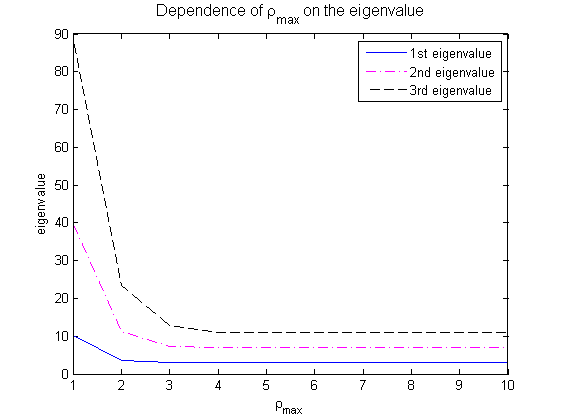
\includegraphics[width=0.75\textwidth]{Figures/rho_maxOnEigenvalue.png}
	\caption{Awesome caption}
	\label{fig:DependenceOnEigenvalue1}
\end{figure}
From the figure that if $\rho_{max} < 3$ the eigenvalues are varying dramatically.
This happens due to neglection ?? of strongly contributing parts of the eigenfunction. 
\fxnote{is this ok??}
\fxnote{comment on the flat part!!}
The $\rho_{max}$ that, with $n=100$, gives the most accurate result for all three of the first eigenvalues is $\rho_{max} = 5$. 
Since this $\rho_{max}$ gives the most accurate result for a relatively small $n$, this is chosen as the optimal $\rho_{max}$ in this and the following sections for this specific problem. 

With this $\rho_{max}$, we wish to find the number of $n$ that gives the first three eigenvalues with four leading digits. 
This optimal $n$ is found by steady increment of $n$, as seen in \fxnote{figref below}.
\begin{figure}[H]
	\centering
	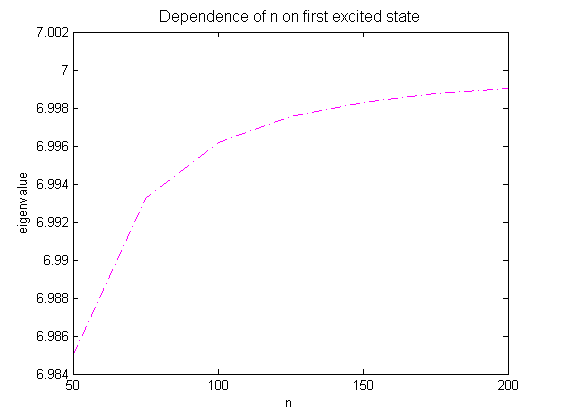
\includegraphics[width=0.75\textwidth]{Figures/MatrixSizeOnEigenvalue_2state.png}
	\caption{Awesome caption}
	\label{fig:DependenceOnEigenvalue2}
\end{figure}
The eigenvalue of the first exited is seen to be asymptotic to the analytical solution $\lambda_1 = 7$, and at a matrix size of $n=200$,  the eigenvalue of the first exited state has the numerical solution $6.99904$. 
This yields an accuracy up to four leading digits, which is also found to be the case for the ground state and the third eigenstate.
Hence, the optimal $\rho_{max}$ and $n$ is $5$ and $200$, respectively. 

	\subsection{Dependence of $n$ on Number of Iterations}
\label{subsec:DependenceOnNumberOfIterations}

In here I want to put the last two figures side by side, but I'm tired now :P
	\chapter{Conclusion}
Conclude.... conclude.... conclude....
 


	% ¤¤ LITTERATURLISTE: SKAL VÆRE SIDST ¤¤
		\bibliographystyle{ieeetr}
		\bibliography{Bibtex/litteratur}

% ¤¤ BILAG: SKAL VÆRE ALLERSIDST ¤¤
	\appendix
	\chapter{MatLab code for smt....}
\label{app:MatLabSolution}
This is how, we write MatLab code in the report
\lstset{language=Matlab}
\begin{lstlisting}
close all
clear all
clc
%I am a comment

filename = 'Results.xlsx';
sheet = 4;
xlRange = 'B3:C12';

[v,T,vT] = xlsread(filename, sheet, xlRange);
x10=v(:,1);y10=v(:,2);

figure
plot(??)
legend(??)

xlim([??])
ylim([??])

title(??)
xlabel('x')
ylabel('y')
\end{lstlisting}

	
\end{document}